\textcolor{red}{Ueberleitung}

\begin{lemma}[Grothendieck's identity]\label{lem:G_id}
	Let $x,y\in\mathbb{R}^d$ be unit vectors. Let $r\in\mathbb{R}^d$ be a random unit vector chosen from $O(d)$-invariant probability distribution on the unit sphere. Then
	\begin{enumerate}
		\item[i,] $\mathbb{P}[\sgn(\sclr{x}{r})\neq\sgn(\sclr{y}{r})]=\frac{\arccos(\sclr{x}{y})}{\pi}$
		\item[ii,] $\mathbb{E}[\sgn(\sclr{x}{r})\sgn(\sclr{y}{r})]=\frac{2}{\pi}\arcsin(\sclr{x}{y}).$
	\end{enumerate}
\end{lemma}
\begin{proof}
	For the proof of $i,$ assume that $x$ and $y$ are linearly dependent. Since both, $x$ and $y$, are unit vectors, $\arccos(\sclr{x}{y}) = \arccos(1)=0$ if $x=y$ or $\arccos(\sclr{x}{y}) = \arccos(-1) = \pi$ if $x=-y$.
	
	
	Conversely assume that $x$ and $y$ are linearly independent, i.\,e. $\operatorname{dim}(\spn\{x,y\})=2$. Now project $r$ orthogonally on the plane spanned by $x$ and $y$. This gives us a vector $s\in \spn\{x,y\}$ with $\sclr{x}{r} = \sclr{x}{s}$ and $\sclr{y}{r} = \sclr{y}{s}$. The unit vector $n\coloneqq s/\norm{s}$ is uniformly distributed on the \textcolor{red}{unit circle/disk} that occurs if we consider the intersection of the unit sphere and $\spn\{x,y\}$ by the $O(d)$-invariance of the probability distribution. \\
	
	\textcolor{red}{Noch naeher auf diese Gleichverteilung eingehen?}
	
	\begin{align*}
		\mathbb{P}[\sgn(\sclr{x}{r})\neq\sgn(\sclr{y}{r})]= \mathbb{P}[\sgn(\sclr{x}{n})\neq\sgn(\sclr{y}{n})] 
	\end{align*} 
	
	\noindent\begin{minipage}{\textwidth}	
		If $n$ lies on the segment of the unit circle induced by the green part, the angle between $x$ and $n$ as well as between $y$ and $n$ is smaller than $\pi/2$, hence $\sclr{x}{n}$ and $\sclr{y}{n}$ are positive. 
		\begin{wrapfigure}{r}{0.4\textwidth}
			\vspace{-20pt}
			\begin{center}
				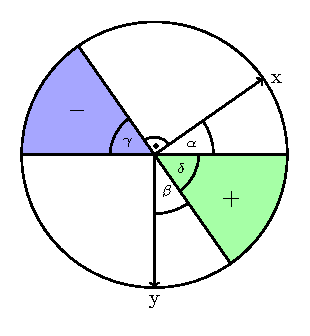
\includegraphics[width=0.38\textwidth]{chapters/fig_unit_circle.pdf}
			\end{center}
			\vspace{-20pt}
		\end{wrapfigure}
		Otherwise, if $n$ lies on the segment of the unit circle induced by the blue part, the angle between both $x$ and $n$ as well as $y$ and $n$ is greater than $3\pi/2$, hence $\sclr{x}{n}$ and $\sclr{y}{n}$ are negative.
		
		\hspace{12pt} Now, if we want to calculate the probability that the signs of the two scalar products disagree, we are interested in the undyed segments of the unit circle. Thus, it is sufficient to calculate the periphery of the undyed segments of the circle. In particular on the unit circle, the angle between two vectors equals the periphery of the segment of the circle between those two vectors. 
			
		\hspace{12pt} Because $\gamma$ and $\delta$ are vertical angles they are both equal. Furthermore, $\alpha$ and $\beta$ have to be equal too, since $\gamma$ and $\delta$ are equal and $\alpha+\delta = \beta+\gamma = \pi/2$. With $\alpha = \arccos(\sclr{x}{y}) - \pi/2$ the first part of Lemma \ref{lem:G_id} follows:
	\end{minipage}
	
	\begin{align*}
		\mathbb{P}[\sgn(\sclr{x}{n})\neq\sgn(\sclr{y}{n})]=2\frac{\frac{\pi}{2}+\alpha}{2\pi} = \frac{\arccos(\sclr{x}{y})}{\pi}.
	\end{align*}
	
	\noindent We conclude with the proof of the second part of Lemma \ref{lem:G_id}: 
	\begin{align*}
		&\mathbb{E}[\sgn(\sclr{x}{r}) \sgn(\sclr{y}{r})] \\
		&\qquad= 1\cdot\mathbb{P}[\sgn(\sclr{x}{r}) = \sgn (\sclr{y}{r} )] - 1\cdot \mathbb{P}[\sgn(\sclr{x}{r}) \neq \sgn(\sclr{y}{r})] \\
		&\qquad= 1 - 2\mathbb{P}[\sgn(\sclr{x}{r}) \neq \sgn(\sclr{y}{r})] \\
		&\qquad= 1 - 2 \frac{\arccos(\sclr{x}{y})}{\pi} \\
		&\qquad= \frac{2}{\pi} \arcsin(\sclr{x}{y}),
	\end{align*}
	because $\arcsin (t) = \arccos(t) = \pi/2$.
\end{proof}

\begin{lemma}[Krivine's trick]\label{lem:krivines_trick}
	Let $x_1,\dots,x_m,y_1,\dots,y_n\in S^{m+n-1}$ be given. Furthermore, let $r\in\mathbb{R}^d$ be a random unit vector chosen form the $O(d)$-invariant probability distribution on the unit sphere. Then there are $x_1^\prime,\dots,x_m^\prime, y_1^\prime,\dots,y_n^\prime\in S^{m+n-1}$ so that
	\begin{equation}
		\mathbb{E}[\sgn(\sclr{x_i^\prime}{r})\sgn(\sclr{y_j^\prime}{r})] = \beta \sclr{x_i}{y_j},
		\label{eq:krivines_trick}
	\end{equation}		
	with $\beta = \frac{2}{\pi} \ln (1+\sqrt{2}).$
\end{lemma}

\noindent For the proof of \ref{lem:krivines_trick} we need to use the $k$-th tensor product of $\mathbb{R}^n$. The $\mathbb{R}^n$ is an $n$-dimensional Euclidean space with inner product \sclr{\cdot}{\cdot} and orthonormal basis $e_1,\dots,e_n$. The \emph{$k$-th tensor product of $\mathbb{R}^n$} is denoted by $(\mathbb{R}^n)^{\tensor k}$ and it is a Euclidean  vector space of dimension $n^k$ with orthonormal basis $e_{i_1}\tensor e_{i_2} \tensor \cdots \tensor e_{i_k}$, $i_j\in\{1,\dots,n\}$. In particular
\begin{align}
	\sclr{e_{i_1}\tensor \cdots \tensor e_{i_k}}{e_{j_1}\tensor \cdots \tensor e_{j_k}}
	&= \prod_{l=1}^k \sclr{e_{i_l}}{e_{j_l}}\nonumber\\
	&=\begin{cases}
		1 & , \text{ if } i_l=j_l \text{ for all } l=1,\dots,n,\\
		0 & , \text{ otherwise},
	\end{cases} \label{eq:orthonormtensor}
\end{align}
and for $v\in\mathbb{R}^n$ with $v=v_1e_1+\cdots +v_ne_n$ we define $v^{\tensor k} \in (\mathbb{R}^n)^{\tensor k}$ by 
\begin{equation}
	v^{\tensor k} = (v_1e_1 + \cdots + v_ne_n) \tensor \cdots \tensor (v_1e_1 + \cdots + v_ne_n) = \sum_{i_1,\dots,i_k} v_{i_1}\cdots v_{i_k} e_{i_1}\tensor\cdots\tensor e_{i_k},
\end{equation}
where the last equation follows by the distributive law (identity $ii,$ of the tensor product). 
Thus, for $v,w\in\mathbb{R}^n$ 
\begin{align}
	\sclr{v^{\tensor k}}{w^{\tensor k}}
%	&\overset{\textcolor{white}{\eqref*{eq:orthonormtensor}}}{=} \sum_{i_1,\dots,i_k} v_{i_1}\cdots v_{i_k}\left(e_{i_1}\tensor\cdots\tensor e_{i_k}\right)^\top \sum_{j_1,\dots,j_k} w_{j_1}\cdots w_{j_k}(e_{j_1}\tensor\cdots\tensor e_{j_k}) \nonumber\\
	&\overset{\textcolor{white}{\eqref*{eq:orthonormtensor}}}{=} \sum_{i_1,\dots,i_k} v_{i_1}\cdots v_{i_k} \sum_{j_1,\dots,j_k} w_{j_1}\cdots w_{j_k} \sclr{e_{i_1}\tensor\cdots\tensor e_{i_k}}{e_{j_1}\tensor\cdots\tensor e_{j_k}} \nonumber\\
	&\overset{\eqref{eq:orthonormtensor}}{=} \sum_{i_1,\dots,i_k} v_{i_1}\cdots v_{i_k}w_{i_1}\cdots w_{i_k} \nonumber\\
	&\overset{\textcolor{white}{\eqref*{eq:orthonormtensor}}}{=}(\sum_{i=1}^n v_iw_i)^k = \sclr{v}{w}^k \label{eq:kth_tensor}
\end{align}
\begin{proof}
	Define the function $E: [-1,+1] \to [-1,+1]$ by $E(t)=\frac{2}{\pi}\arcsin(t)$. Due to Grothendieck's identity (Lemma \ref{lem:G_id}):
	\begin{align*}
		E(\sclr{x_i^\prime}{y_j^\prime} ) &= \mathbb{E}[\sgn(\sclr{x_i^\prime}{r})\sgn(\sclr{y_j^\prime}{r})]\\
		&\overset{!}{=}\beta \sclr{x_i}{y_j}.
	\end{align*}
	
	\noindent Idea: To find $\beta,x_i^\prime,y_j^\prime$ we invert $E$:
	\[
		\sclr{x_i^\prime}{y_j^\prime} = E^{-1} (\beta \sclr{x_i}{y_j})	
	\]
	with 
	\begin{align*}
		E^{-1}(t) &= \sin(\pi/2 \cdot t) \\
		&= \sum_{k=0}^\infty \underbrace{\frac{(-1)^{2k+1}}{(2k+1)!}\left(\frac{\pi}{2}\right)^{2k+1}}_{g_{2k+1}}  t^{2k+1}
	\end{align*}
	which is valid for all $t\in[-1,+1]$.
	
	Define the infinite-dimensional Hilbert space
	\begin{equation}
		H= \bigoplus_{r=0}^\infty (\mathbb{R}^{m+n})^{\tensor 2k+1}.
	\end{equation}
	\textcolor{red}{Begruenden, dass H gross genug ist?}
	
	Define $\tilde{x}_i, \tilde{y}_j\in H$, $i=1,\dots,m,j=1,\dots,n$ componentwise:
	\begin{align*}
		(\tilde{x}_i)_k &= \sgn(g_{2k+1}) \sqrt{\modul{g_{2k+1}}\beta^{2k+1}}\, x_i^{\tensor 2k+1} \\
		(\tilde{y}_j)_k &= \sqrt{\modul{g_{2k+1}}\beta^{2k+1}} \,y_j^{\tensor 2k+1}
	\end{align*}
	Then 
	\begin{align*}
		\sclr{\tilde{x}_i}{\tilde{y}_j} &\overset{\textcolor{white}{\eqref*{eq:kth_tensor}}}{=} \sum_{k=0}^\infty g_{2k+1} \beta^{2k+1}\sclr{x_i^{\tensor 2k+1}}{y_j^{\tensor 2k+1}} \\
		&\overset{\eqref{eq:kth_tensor}}{=} \sum_{k=0}^\infty g_{2k+1} \beta^{2k+1} \sclr{x_i}{y_j}^{2k+1} \\
		&\overset{\textcolor{white}{\eqref*{eq:kth_tensor}}}{=} E^{-1}(\beta \sclr{x_i}{y_j}).
	\end{align*}
	
	Hence, $\beta$ is defined by the condition that the vectors $\tilde{x}_i,\dots,\tilde{x}_m,\tilde{y}_1,\dots,\tilde{y}_n$ are unit vectors, that is
	\[
		1 = \sclr{\tilde{x}_i}{\tilde{x}_i} = \sclr{\tilde{y}_j}{\tilde{y}_j}
		%= \sum_{k=0}^\infty \modul{g_{2k+1}} \beta^{2k+1} 
		= \sum_{k=0}^\infty \frac{1}{(2k+1)!}\left(\frac{\pi}{2}\right)^{2k+1}\beta^{2k+1}=\sinh(\frac{\pi}{2}\beta).
	\]
	Consequently
	\[
		\beta = \frac{2}{\pi} \arcsinh(1) = \frac{2}{\pi}\ln(1+\sqrt(2)),	
	\]
	since $\arcsinh (t) = \ln(t+\sqrt{t^2+1})$.

	The only thing that is left to prove, is that the solution of the maximization problem yields vectors $x_1^\prime,\dots,x_m^\prime, y_1^\prime,\dots,y_n^\prime\in S^{m+n-1}$, since our vectors $\tilde{x}_1,\dots,\tilde{x}_m,\tilde{y}_1,\dots,\tilde{y}_n$ are infinite-dimensional. 
	For this reason consider the real matrix $G\in\mathbb{R}^{(m+n)\times(m+n)}$ given by
	\begin{equation}
		G=\begin{pmatrix}
			\sclr{\tilde{x}_1}{\tilde{x}_1} & \cdots & \sclr{\tilde{x}_1}{\tilde{x}_m}& \sclr{\tilde{x}_1}{\tilde{y}_1} & \cdots & \sclr{\tilde{x}_1}{\tilde{y}_n} \\
			 \vdots		& \ddots	& \vdots & \vdots & \ddots & \vdots\\
			 \sclr{\tilde{x}_m}{\tilde{x}_1} & \cdots & \sclr{\tilde{x}_m}{\tilde{x}_m}& \sclr{\tilde{x}_m}{\tilde{y}_1} & \cdots & \sclr{\tilde{x}_m}{\tilde{y}_n} \\
			\sclr{\tilde{y}_1}{\tilde{x}_1} & \cdots & \sclr{\tilde{y}_1}{\tilde{x}_m}& \sclr{\tilde{y}_1}{\tilde{y}_1} & \cdots & \sclr{\tilde{y}_1}{\tilde{y}_n} \\
			 \vdots		& \ddots	& \vdots& \vdots & \ddots & \vdots\\
			 \sclr{\tilde{y}_n}{\tilde{x}_1} & \cdots & \sclr{\tilde{y}_n}{\tilde{x}_m}& \sclr{\tilde{y}_n}{\tilde{y}_1} & \cdots & \sclr{\tilde{y}_n}{\tilde{y}_n} 
		\end{pmatrix}
	\end{equation}
	called \emph{Gram matrix}. Let $z\coloneqq (\tilde{x}_1,\dots,\tilde{x}_m,\tilde{y}_1,\dots,\tilde{y}_n)$. By the linearity of the scalar product
	\begin{align*}
		v^\top G v = \sum_{i,j} v_i G_{ij} v_j 
		= \sum_{i,j} v_i \sclr{z_i}{z_j} v_j 
		= \sclr{\sum_i v_i z_i}{\sum_j v_j z_j} 
		= \norm{\sum_i v_i z_i} > 0
	\end{align*}
	for some $v\in\mathbb{R}^{m+n}$, $v\neq 0$. Hence, $G$ is positive definite and symmetric, thus, $G$ can be diagonalized by an orthogonal matrix. This means that there is a decomposition $G=Q\Lambda Q^\top$ with $Q$ a real orthogonal matrix with columns that are the eigenvectors of $G$ and $\Lambda$ a real and diagonal matrix having the eigenvalues of $G$ on the diagonal. Since the eigenvalues of a positive definite matrix are positive, $\Lambda=\Lambda^{1/2}\Lambda^{1/2}$. Thus,
	\[
		G=(Q\Lambda^{1/2})(Q\Lambda^{1/2})^\top		
	\]
	and due to the symmetry of $G$ likewise
	\[
		G=(Q\Lambda^{1/2})^\top(Q\Lambda^{1/2}).	
	\]
	$A\coloneqq Q\Lambda^{1/2}$ is a real $(m+n)\times (m+n)$ matrix and its columns are the vectors we were looking for.
	\textcolor{red}{Muss man hier dann noch begruenden, dass die Vektoren immer noch Einheitsvektoren sind? Oder muss das der Fall sein, sonst hätte man ja nicht immer eine 1 auf der Diagonalen und folglich nicht die selbe Matrix?}
\end{proof}
\begin{dfn}
	For $M\in\mathbb{R}^{m\times n}$ define the quadratic program \textcolor{red}{wieso quadratisch?}
	\begin{align}
		\norm{M}_{\infty\to 1} &= \max \left\{ \sum_{i=1}^m \sum_{j=1}^n M_{ij} \xi_i \eta_j : \xi_i^2=1, i=1,\dots,m, \eta_j^2=1, j =1,\dots,n \right\} \\
		&=\max\left\{\trace{\xi^\top M \eta}: \xi\in\{-1,1\}^m,\eta\in\{-1,1\}^n\right\}.
	\end{align}
\end{dfn}
\textcolor{red}{computing NP-hard}
\begin{dfn}
	\textcolor{red}{sdp relaxation einfuehren}
	
	SDP relaxation of $\norm{M}_{\infty\to1}$:
	\begin{align*}
		\operatorname{sdp}_{\infty\to 1} (M) = \max 
		&\sum_{i=1}^m\sum_{j=1}^n M_{ij} \sclr{x_i}{y_j}\\
		&x_i,y_j\in\mathbb{R}^{m+n}\\
		&\norm{x_i}=1, i=1,\dots,m\\
		&\norm{y_j}=1, j=1,\dots,n.
	\end{align*}
\end{dfn}
\begin{theo}[Grothendieck's inequality] \label{theo:G_ineq}
	There exists a constant $K$ such that for all $M\in\mathbb{R}^{m\times n}$:
	\begin{equation}
		\norm{M}_{\infty\to 1} \leq \operatorname{sdp}_{\infty\to 1} (M) \leq K \norm{M}_{\infty\to 1}.
	\end{equation}
\end{theo}
\begin{proof}
	\textcolor{red}{wieso again? wo wurde das vorher schon einmal gemacht?}
	Again: approximation algorithm with randomized rounding
	
	\begin{algorithm}[H]
		\SetAlgoLined
		\caption{Approximation algorithm with randomized rounding for $\norm{M}_{\infty\to 1}$}
	\end{algorithm}
	\begin{itemize}
		\item[1.] Solve $\operatorname{sdp}_{\infty\to 1} (M)$. Let $x_1,\dots,x_m,y_1,\dots,y_n\in S^{m+n-1}$ be the optimal unit vectors
		\item[2.] Apply Krivine's trick (Lemma \ref{lem:krivines_trick}) and use vectors $x_i,y_j$ to create new unit vectors $x_1^\prime,\dots,x_m^\prime, y_1^\prime,\dots,y_n^\prime\in S^{m+n-1}$.
		\item[3.] Choose $r\in S^{m+n-1}$ randomly
		\item[4.] Round: $u_i = \sgn(\sclr{x_i^\prime}{r})$\\
					\textcolor{white}{Round: }$v_j = \sgn(\sclr{y_j^\prime}{r})$
	\end{itemize}
	
	\noindent Expected quality of the outcome:
	\begin{align*}
		\norm{M}_{\infty\to 1} &\geq \mathbb{E}\left[\sum_{i=1}^m\sum_{j=1}^n M_{ij}u_iv_j\right]\\
		&\overset{\textcolor{white}{\eqref*{eq:krivines_trick}}}{=} \sum_{i=1}^m\sum_{j=1}^n M_{ij} \mathbb{E}[\sgn(\sclr{x_i^\prime}{r}) \sgn(\sclr{y_j^\prime}{r})] \\
		&\overset{\textcolor{white}{\eqref*{eq:krivines_trick}}}{=}\sum_{i=1}^m\sum_{j=1}^n M_{ij}\beta \sclr{x_i}{y_j} \\
		&\overset{\eqref{eq:krivines_trick}}{=}\beta \operatorname{sdp}_{\infty\to 1}(M),
	\end{align*}
	where $\beta = \frac{2\ln(1+\sqrt(2)}{\pi}$, thus $K_G\leq \beta^{-1}$.
\end{proof}

\begin{theo}[Grothendieck-Tsirelson]
	There exists an absolute constant $K\geq 1$ such that, for any positive integers $m,n$, the following three equivalent conditions hold:
	\begin{itemize}
		\item[(1)] We have the inclusion 
			\begin{equation}
				\QC_{m,n} \subset K\LC_{m,n}.
			\end{equation}
		\item[(2)] For any $M\in\mathbb{R}^{m\times n}$ and for any $\rho,X_i,Y_j$ verifying the conditions of Definition \textcolor{red}{4.2.1} we have
			\begin{equation}
				\sum_{i,j} M_{ij} \trace{\rho(X_i\tensor Y_j)}\leq K \max_{\xi\in\{-1,1\}^m,\eta\in\{-1,1\}^n} \trace{\xi^\top M \eta}.
			\end{equation}
			\item[(3)] For any $M\in\mathbb{R}^{m\times n}$ and for any (real) Hilbert space vectors $x_i,y_j$ with $\modul{x_i}\leq 1$, $\modul{y_j}\leq 1$ we have
				\begin{equation}
					\sum_{i,j} M_{i,j}\sclr{x_i}{y_j} \leq K \max_{\xi\in\{-1,1\}^m,\eta\in\{-1,1\}^n} \trace{\xi^\top M \eta}. \label{eq:G_ineq}
				\end{equation}
	\end{itemize}
\end{theo}
\begin{proof}
	Since \eqref{eq:G_ineq} is a direct consequence of Grothendieck's inequality the only thing left to prove is the equivalence between (1)-(3). The equivalence of (3) and (2) (the Tsirelson's bound) is a consequence of \textcolor{red}{the proof of Lemma \textcolor{red}{4.2.2}, where we proved that $\trace{\rho(X_i\tensor Y_j)} = \sclr{x_i}{y_j}$.}
	\textcolor{red}{Dann brauchen wir hier noch Argumente aus Exercise 11.3.}
	Finally, the equivalence between (2) and (1) ...
\end{proof}
\newpage